\subsection{Prototipo mínimo viable}
El proyecto tiene como finalidad desarrollar una pagina web que ofrezca recomendaciones confiables y enfocados en la seguridad y comodidad de los nómadas digitales que se encuentran en Bogotá. El desarrollo se llevará a cabo usando arquitecturas y herramientoas que den pie a la creación de
una plataforma sostenible, escalable y dispuesta a las necesidades de los usuarios, primando la experiencia del usuario a traves de la seguridad y confianza en la información que se le brinda.

\textbf{Tecnologías}
\begin{itemize}
    \item \textbf{Spring Boot: } Spring Boot es un framework de desarrollo de aplicaciones Java que simplifica la creación de aplicaciones empresariales. Proporciona una configuración automática y una amplia gama de herramientas para facilitar el desarrollo, lo que permite a los desarrolladores centrarse en la lógica del negocio en lugar de la configuración del entorno.
    Spring Boot es especialmente útil para crear aplicaciones web y servicios RESTful, ya que incluye características como la gestión de dependencias, la configuración de seguridad y la integración con bases de datos. Además, permite el despliegue rápido de aplicaciones en entornos de producción, lo que lo convierte en una opción popular para el desarrollo ágil.
    \vspace{2mm}
    \begin{minipage}{0.9\textwidth}
        \centering
        \captionof{figure}[{Logo Spring Boot}]{ Logo Spring Boot  }
        \label{Firestore}
         
\includegraphics[width=0.3\textwidth]{Content/Images/spring-boot-logo.png}
        \footnote{Nota. \textup{Fuente: spring.io}}
    \end{minipage}

    \item \textbf{Angular: } Angular es un framework web que permite a los desarrolladores crear aplicaciones rápidas y fiables.
    Mantenido por un equipo dedicado de Google, Angular ofrece un amplio conjunto de herramientas, API y bibliotecas para simplificar y optimizar tu flujo de trabajo de desarrollo. Angular te ofrece una plataforma sólida para crear aplicaciones rápidas y fiables que escalan con el tamaño de tu equipo y de tu código fuente.

    Angular es muy util para el desarrollo de aplicaciones web modernas, ya que permite crear interfaces de usuario dinámicas y reactivas. Su enfoque basado en componentes facilita la reutilización del código y mejora la mantenibilidad de las aplicaciones. Además, Angular cuenta con un ecosistema robusto que incluye herramientas para pruebas, enrutamiento y gestión del estado, lo que lo convierte en una opción popular para el desarrollo de aplicaciones empresariales.
    
    \vspace{2mm}
    \begin{minipage}{0.9\textwidth}
        \centering
        \captionof{figure}[{Logo Angular}]{Logo Angular}
        \label{angularLogo}
        
\includegraphics[width=0.25\textwidth]{Content/Images/angular-logo.png}
        \footnote{Nota. \textup{Fuente: angular.io}}
    \end{minipage}
    
    \item \textbf{PostgreSQL: } PostgreSQL es un potente sistema de base de datos relacional de objetos de código abierto con más de 35 años de desarrollo activo eso le ha valido una sólida reputación de confiabilidad, robustez de características y rendimiento.

    La comunidad de código abierto proporciona muchos lugares útiles para familiarizarse con PostgreSQL, incluyendo la documentación oficial, tutoriales y foros de discusión. PostgreSQL es conocido por su capacidad para manejar grandes volúmenes de datos y transacciones complejas, lo que lo convierte en una opción popular para aplicaciones empresariales y sistemas de gestión de datos críticos.
    \vspace{2mm}
    \begin{minipage}{0.9\textwidth}
        \centering
        \captionof{figure}[{Logo PostgreSQL}]{Logo PostgreSQL}
        \label{postgresqlLogo}
        
\includegraphics[width=0.3\textwidth]{Content/Images/postgresql-logo.png}
        \footnote{Nota. \textup{Fuente: postgresql.org}}
    \end{minipage}

\end{itemize}

\vspace{5mm}
\textbf{Arquitectura} 

\begin{itemize}
    \item\textbf{Arquitectura de microservicios: }Los microservicios son una arquitectura de software donde la aplicación se divide en pequeños servicios independientes, cada uno con una función específica (ej.: autenticación, procesamiento de pagos, geolocalización), que se comunican entre sí mediante APIs. A diferencia de las aplicaciones monolíticas, cada microservicio puede desarrollarse, desplegarse y escalarse por separado, usando tecnologías distintas según su necesidad.
    Esta arquitectura permite escalar selectivamente funciones críticas (como alertas en tiempo real o validación de zonas), integrar tecnologías diversas y aislar fallos sin colapsar todo el sistema. Además, facilita la expansión modular a nuevas ciudades y optimiza costos en la nube al escalar solo lo necesario
    \vspace{2mm}
    \begin{minipage}{0.9\textwidth}
        \centering
        \captionof{figure}[{Arquitectura de Microservicios.}]{Ejemplo de arquitectura de microservicios.}
        \label{microservicios}
        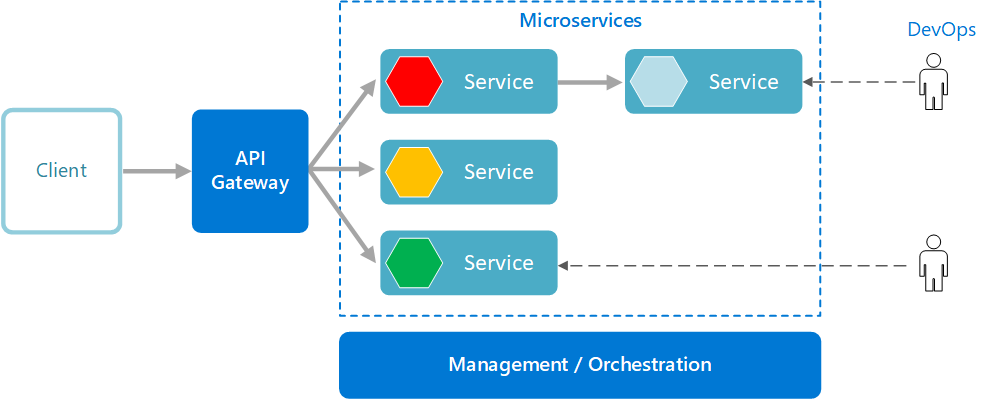
\includegraphics[width=0.3\textwidth]{Content/Images/microservices-logical.png}
        \footnote{Nota. \textup{Fuente: learn.microsoft.com/es-es/azure/architecture/guide/architecture-styles/microservices}}
    \end{minipage}
%------------------------------------------------------------------%


{\color{red}

\textbf{Arquitectura} 
\begin{itemize}
    
    \item \textbf{Arquitectura de microservicios: } La arquitectura de microservicios es un enfoque de desarrollo de aplicaciones que divide el software en pequeños servicios independientes, cada uno enfocado en realizar una función específica del negocio. Estos microservicios funcionan de manera autónoma y pueden estar desarrollados en diferentes lenguajes de programación. Se comunican entre sí a través de APIs y, en muchos casos, utilizan su propio sistema de almacenamiento, lo que contribuye a la estabilidad y escalabilidad de la aplicación al evitar sobrecargas y puntos únicos de fallo.
    
    Este enfoque ha sido seleccionado para la arquitectura del back-end, ya que facilita la implementación modular de los servicios necesarios para el negocio. Además, permite que cada servicio se despliegue de manera independiente, lo cual es ideal para su posterior despliegue en plataformas como Firebase.
    
    \vspace{2mm}
    \begin{minipage}{0.9\textwidth}
        \centering
        \captionof{figure}[{Arquitectura de Microservicios.}]{Ejemplo de arquitectura de microservicios.}
        \label{microservicios}
        
\includegraphics[width=0.3\textwidth]{Content/Images/Escudo_UD.png}
        \footnote{Nota. \textup{Fuente: decidesoluciones.es/arquitectura-de-microservicios}}
    \end{minipage}
    
    \item \textbf{Arquitectura hexagonal: } La Arquitectura Hexagonal, también conocida como Arquitectura de Puertos y Adaptadores, es un patrón de diseño propuesto por Alistair Cockburn, que organiza el software en capas con el objetivo de aislar cada funcionalidad, permitiendo una evolución más ordenada y modular del sistema. El núcleo de esta arquitectura es el dominio, y cada lado del hexágono representa una interacción con servicios externos, facilitando así la integración y adaptabilidad a futuros cambios.
    
    Esta arquitectura permite que los componentes del sistema se mantengan independientes unos de otros, facilitando el mantenimiento y la escalabilidad. En este caso, el dominio principal se mantiene aislado mientras que los adaptadores interactúan con bases de datos, APIs, y otros servicios externos.
    
    \vspace{2mm}
    \begin{minipage}{0.9\textwidth}
        \centering
        \captionof{figure}[{Arquitectura Hexagonal.}]{Ejemplo de arquitectura hexagonal.}
        \label{hexagonal}
        
\includegraphics[width=0.3\textwidth]{Content/Images/Escudo_UD.png}
        \footnote{Nota. \textup{Fuente: https://softwarecrafters.io/react/arquitectura-hexagonal-frontend}}
    \end{minipage}

    
\end{itemize}

\textbf{Infraestructura }
\newline
La computación en la nube sigue siendo un componente fundamental de este proyecto, permitiendo la entrega y uso de almacenamiento, servidores, aplicaciones y otros recursos a través de Internet, bajo un modelo de pago por consumo. En lugar de depender de centros de datos locales o infraestructuras físicas, la infraestructura utilizada se apoya en servicios remotos y gestionados, lo que permite una escalabilidad eficiente y una gestión optimizada de los recursos.

Para este proyecto, se ha seleccionado Firebase como plataforma en la nube. Firebase ofrece una infraestructura integral que facilita el desarrollo y despliegue de aplicaciones, proporcionando servicios como bases de datos en tiempo real, almacenamiento, autenticación y hosting, todos gestionados de manera centralizada. Esto elimina la necesidad de administrar servidores físicos o realizar configuraciones complejas, ya que la plataforma maneja estos aspectos, permitiendo que el desarrollo se enfoque exclusivamente en la creación de la aplicación. \cite{FirebaseCloud}.
\newline
\textbf{Software as a Service (SaaS) :}
El modelo SaaS (Software como Servicio) se utiliza de manera prominente en este proyecto, ya que Firebase funciona bajo este esquema. Firebase, al ser un servicio gestionado, permite a los desarrolladores centrarse en el desarrollo del software sin tener que preocuparse por la administración de servidores, las actualizaciones de seguridad o la gestión de licencias. Los usuarios finales pueden acceder a la aplicación y sus funcionalidades desde cualquier ubicación con una conexión a Internet, lo que simplifica tanto el uso como la operación del sistema. \cite{FirebaseSAAS}


\textbf{Requerimientos}

\begin{enumerate}
    \item Funcionales
        \par\vspace{2mm}
        \begin{minipage}{0.9\textwidth}
        \centering
        \captionof{table}[{Requerimiento funcional RF-001.}]{ Requerimiento funcional RF-001. }
        \label{req1}
        
\includegraphics[width=0.3\textwidth]{Content/Images/Escudo_UD.png}
        \footnote{}{Nota. \textup{Fuente : Autores.}}
        \end{minipage}
        
        \vspace{2mm}
        \begin{minipage}{0.9\textwidth}
        \centering
        \captionof{table}[{Requerimiento funcional RF-002.}]{ Requerimiento funcional RF-002. }
        \label{req2}
        
\includegraphics[width=0.3\textwidth]{Content/Images/Escudo_UD.png}
        \footnote{}{Nota. \textup{Fuente : Autores.}}
        \end{minipage}
        
        \vspace{2mm}
        \begin{minipage}{0.9\textwidth}
        \centering
        \captionof{table}[{Requerimiento funcional RF-003.}]{ Requerimiento funcional RF-003. }
        \label{req3}
        
\includegraphics[width=0.3\textwidth]{Content/Images/Escudo_UD.png}
        \footnote{}{Nota. \textup{Fuente : Autores.}}
        \end{minipage}
        
        \vspace{2mm}
        \begin{minipage}{0.9\textwidth}
        \centering
        \captionof{table}[{Requerimiento funcional RF-004.}]{ Requerimiento funcional RF-004. }
        \label{req4}
        
\includegraphics[width=0.3\textwidth]{Content/Images/Escudo_UD.png}
        \footnote{}{Nota. \textup{Fuente : Autores.}}
        \end{minipage}
        
        \vspace{2mm}
        \begin{minipage}{0.9\textwidth}
        \centering
        \captionof{table}[{Requerimiento funcional RF-005.}]{ Requerimiento funcional RF-005. }
        \label{req5}
        
\includegraphics[width=0.3\textwidth]{Content/Images/Escudo_UD.png}
        \footnote{Nota. \textup{Fuente : Autores.}}
        \end{minipage}
        
        \vspace{2mm}
    %    \begin{minipage}{0.9\textwidth}
    %    \centering
    %    \captionof{table}[{Requerimiento funcional RF-006.}]{ Requerimiento funcional RF-006. }
    %    \label{req6}

    %    \end{minipage}
        

        
    \item No funcionales
    
        
        \vspace{2mm}
        \begin{minipage}{0.9\textwidth}
        \centering
        \captionof{table}[{Requerimiento no funcional RNF-001.}]{ Requerimiento no funcional RNF-001. }
        \label{reqnf1}
         
\includegraphics[width=1\textwidth]{Content/Images/Escudo_UD.png}
        \footnote{Nota. \textup{Fuente : Autores.}}
        \end{minipage}
        
        \vspace{2mm}
        \begin{minipage}{0.9\textwidth}
        \centering
        \captionof{table}[{Requerimiento no funcional RNF-002.}]{ Requerimiento no funcional RNF-002. }
        \label{reqnf2}
        
\includegraphics[width=1\textwidth]{Content/Images/Escudo_UD.png}
        \footnote{Nota. \textup{Fuente : Autores.}}
        \end{minipage}

        \vspace{2mm}
        \begin{minipage}{0.9\textwidth}
        \centering
        \captionof{table}[{Requerimiento no funcional RNF-003.}]{ Requerimiento no funcional RNF-003. }
        \label{reqnf3}
        
\includegraphics[width=1\textwidth]{Content/Images/Escudo_UD.png}
        \footnote{}{Nota. \textup{Fuente : Autores.}}
        \end{minipage}
        
\end{enumerate}

\textbf{Casos de uso}
    
    \vspace{2mm}
    \begin{minipage}{0.9\textwidth}
    \centering
    \captionof{figure}[{Caso de uso RF-001.}]{ Caso de uso RF-001. }
    \label{caso1}
    
\includegraphics[width=0.3\textwidth]{Content/Images/Escudo_UD.png}
    \footnote{Nota. \textup{Fuente : Autores.}}
    \end{minipage}
    
    \vspace{2mm}
    \begin{minipage}{0.9\textwidth}
    \centering
    \captionof{figure}[{Caso de uso RF-002.}]{ Caso de uso RF-002. }
    \label{caso2}
    
\includegraphics[width=0.3\textwidth]{Content/Images/Escudo_UD.png}
    \footnote{Nota. \textup{Fuente : Autores.}}
    \end{minipage}
    
    \vspace{2mm}
    \begin{minipage}{0.9\textwidth}
    \centering
    \captionof{figure}[{Caso de uso RF-003.}]{ Caso de uso RF-003. }
    \label{caso3}
    
\includegraphics[width=0.3\textwidth]{Content/Images/Escudo_UD.png}
    \footnote{Nota. \textup{Fuente : Autores.}}
    \end{minipage}
    
    \vspace{2mm}
    \begin{minipage}{0.9\textwidth}
    \centering
    \captionof{figure}[{Caso de uso RF-004.}]{ Caso de uso RF-004. }
    \label{caso4}
    
\includegraphics[width=0.3\textwidth]{Content/Images/Escudo_UD.png}
    \footnote{Nota. \textup{Fuente : Autores.}}
    \end{minipage}
    
    \vspace{2mm}
    \begin{minipage}{0.9\textwidth}
    \centering
    \captionof{figure}[{Caso de uso RF-005.}]{ Caso de uso RF-005. }
    \label{caso1}
    
\includegraphics[width=0.3\textwidth]{Content/Images/Escudo_UD.png}
    \footnote{Nota. \textup{Fuente : Autores.}}
    \end{minipage}
    


\textbf{Vistas principales del prototipo}
De acuerdo a los requerimientos funcionales y no funcionales junto con los casos de uso, a continuación, en las figuras \ref{prot1}, \ref{prot2}, \ref{prot3}, \ref{prot4}, \ref{prot5}, \ref{prot6}, \ref{prot7}, \ref{prot8}, se adjuntan las vistas que representan el núcleo del plan de negocio. Todas las ilustraciones utilizadas en la creación de este prototipo fueron generadas y desarrolladas específicamente para el presente proyecto.

Los manuales para la instalación y el uso de este prototipo se pueden encontrar en los anexos del documento:
\begin{itemize}
    \item \hyperref[manual-usuario]{Manual de Usuario}
    \item \hyperref[manual-instalacion]{Manual de Instalación}
    \item \hyperref[manual-despliegue]{Manual de Despliegue en Vercel}
\end{itemize}


    \vspace{2mm}
    \begin{minipage}{0.9\textwidth}
    \centering
    \captionof{figure}[{Vista principal}]{ Vista principal }
    \label{prot1}
    
\includegraphics[width=0.3\textwidth]{Content/Images/Escudo_UD.png}
    \footnote{Nota. \textup{Fuente: Autores}}
    \end{minipage}
    
      \vspace{2mm}
    \begin{minipage}{0.9\textwidth}
    \centering
    \captionof{figure}[{Vista nosotros}]{ Vista nosotros }
    \label{prot2}
    
\includegraphics[width=0.3\textwidth]{Content/Images/Escudo_UD.png}
    \footnote{Nota. \textup{Fuente: Autores}}
    \end{minipage}
    
    \vspace{2mm}
    \begin{minipage}{0.9\textwidth}
    \centering
    \captionof{figure}[{Vista registro}]{ Vista registro }
    \label{prot3}
    
\includegraphics[width=0.3\textwidth]{Content/Images/Escudo_UD.png}
    \footnote{Nota. \textup{Fuente: Autores}}
    \end{minipage}
    
    \vspace{2mm}
    \begin{minipage}{0.9\textwidth}
    \centering
    \captionof{figure}[{Vista registro}]{ Vista registro }
    \label{prot4}
    
\includegraphics[width=0.3\textwidth]{Content/Images/Escudo_UD.png}
    \footnote{Nota. \textup{Fuente: Autores}}
    \end{minipage}
    
    \vspace{2mm}
    \begin{minipage}{0.9\textwidth}
    \centering
    \captionof{figure}[{Vista mi progreso}]{ Vista mi progreso }
    \label{prot5}
    
\includegraphics[width=0.3\textwidth]{Content/Images/Escudo_UD.png}
    \footnote{Nota. \textup{Fuente: Autores}}
    \end{minipage}
    
        \vspace{2mm}
    \begin{minipage}{0.9\textwidth}
    \centering
    \captionof{figure}[{Vista eventos}]{ Vista eventos }
    \label{prot6}
    
\includegraphics[width=0.3\textwidth]{Content/Images/Escudo_UD.png}
    \footnote{Nota. \textup{Fuente: Autores}}
    \end{minipage}

        \vspace{2mm}
    \begin{minipage}{0.9\textwidth}
    \centering
    \captionof{figure}[{Vista gimnasios}]{ Vista gimnasios }
    \label{prot7}
    
\includegraphics[width=0.3\textwidth]{Content/Images/Escudo_UD.png}
    \footnote{Nota. \textup{Fuente: Autores}}
    \end{minipage}

    \vspace{2mm}
    \begin{minipage}{0.9\textwidth}
    \centering
    \captionof{figure}[{Vista mis datos}]{ Vista mis datos }
    \label{prot8}
    
\includegraphics[width=0.3\textwidth]{Content/Images/Escudo_UD.png}
    \footnote{Nota. \textup{Fuente: Autores}}
    \end{minipage}


    
    
    

}